\documentclass{article}

\usepackage[margin=1in]{geometry}
\usepackage{amsmath,amssymb}
\usepackage{lscape}
\usepackage{graphicx}
\usepackage{appendix}
\usepackage[center]{caption}

\newcommand{\HRule}{\rule{\linewidth}{0.1mm}}
%\renewcommand{\thesection}{\arabic{section}.}
%\renewcommand{\thesubsection}{\arabic{section}.\arabic{subsection}}

\begin{document}

\title{ \HRule \\[0.2cm]
		Autonomous Agents\\ 
		Report Assignment 1: Single Agent Planning\\
		\HRule \\[0.1cm]
		}
		
\author{
		\emph{Authors:}\\[0.2cm]
		Agnes \textsc{van Belle} \small{ \emph{(10363130)}},\\ 
		Maaike \textsc{Fleuren} \small{ \emph{(10350470)}}, \\
		Norbert \textsc{Heijne} \small{ \emph{(10357769)}}, \\
		Lydia \textsc{Mennes} \small{ \emph{(10333843)}}
		}

 
\maketitle

\section{Introduction}
This report has been written for the Master Artificial Intelligence course Autonomous Agents. This report will contain the answers, motivation and explanation for our implementations of the tasks we had to accomplish in our first assignment for this course. These taks were centered around the topic of ``Single Agent Planning''. 

\subsection{The Environment}\label{environment}
In all tasks there is assumed to be a grid world (of $11 \times 11$) with a predator and a prey in it. The agents can both move one tile forward each iteration. The direction they take (or if they move at all) is affected by probabilities (their policies). If they move over the edge of the grid they end up at the opposing side of the grid. The prey will never step into the predator. We are focused on improving the decisions of one agent, the predator. 



\section{Simulating the environment}
A first task was to write a simulator for the environment as defined in Section \ref{environment}.

The choice has been made to not encode the positions of the agents as part of a grid, i.e. matrix. Instead the agents both know their own position and on each iteration the position of the other agent is given as input by the environment, as we have stated in the Agent interface. This is needed for prey to see if the predator is next to it, to prevent it moving towards the prey. In the predator's case it might be necessary later on to know the position of the prey although it is not necessary for this particular sub-assignment.

As part of the assignment a mean and a standard deviation was asked for 100 runs with the use of the random policy for the predator's behaviour. For the exact output, one can consult Appendix \ref{app:firstMust}. The lowest amount of time steps observed was 19 time steps. The optimal amount of time steps given that the prey would remain still throughout the trial run would be 10. The highest amount observed was 1194 steps. The average amount of time steps was 296.93 time steps and the standard deviation was 244.55 time steps (rounded up). This is a clear indication of the inefficiency of the random policy in this particular setting. 


\section{Planning for the Environment}
It is possible for the predator to develop a more sophisticated policy by planning. Given that that the whole environment is known to the agent, we can make use of several dynamic programming planning algorithms, and we will discuss our implementtaion of these in the subsections below.

\subsection{ Policy Evaluation}
The algorithm for Policy Evaluation follows from turning the Bellman equation into an update rule, such that each iteration of Policy Evaluation, Equation \ref{eq:policyEvaluation} is used for every $s \in \mathcal S$ (where $\mathcal S$ denotes the set of states).
\begin{equation}\label{eq:policyEvaluation}
V_{k+1}(s) \leftarrow \sum_{a} \pi (s,a) \sum_{s'}  \mathcal P_{s s'}^{a} \left( \mathcal R_{s s'}^{a} 
+ \gamma V_{k}(s') \right) 
\end{equation}
Because we used the random policy for the predtaor, and there were five actions possible for the predator, Equation \ref{eq:policyEvaluation} could be simplified to Equation \ref{eq:policyEvaluationSimpler}.
\begin{equation}\label{eq:policyEvaluationSimpler}
V_{k+1}(s) \leftarrow \frac{1}{5} \sum_{a}  \sum_{s'}  \mathcal P_{s s'}^{a} \left( \mathcal R_{s s'}^{a} 
+ \gamma V_{k}(s') \right) 
\end{equation}
Where $\mathcal P_{s s'}^{a}$ has to take into account the possible movements of the prey. Note that $\mathcal R_{s s'}^{a}$ was always zero, except for the single goal state.

We implemented Policy Evaluation using a $121 \times 121$ matrix to hold the $V$- values for the states. 
It took $111$ iterations to converge using $\theta = 0$ and $\gamma = 0.8$.

In the following list we show some values that Policy Evaluation found for specific states:
\begin{itemize}\label{list:policyEvaluationListValues}
\item{\textbf{Predator(0,0), Prey(5,5)}}: $0.0060$		
\item{\textbf{Predator(2,3), Prey(5,4)}}: $0.1820$
\item{\textbf{Predator(2,10), Prey(10,0)}}: $0.1820$
\item{\textbf{Predator(10,10), Prey(0,0)}}: $1.1950$
\end{itemize}


\begin{figure}[htb]\label{colormapPolicyEvaluation}
		\centering
        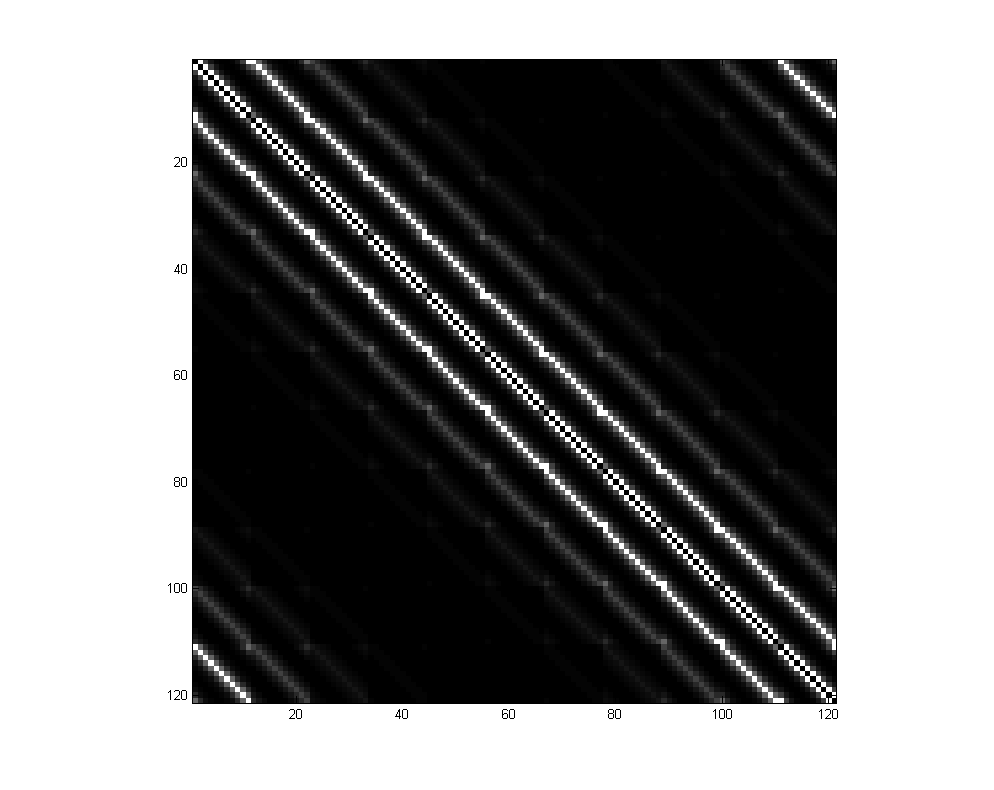
\includegraphics[width=0.9\textwidth]{VMatrixPolicyEvaluation.png}
        \caption{	 Colormap of the $V$-values resulting from Policy Evaluation for
        			 $\theta=0$ and $\gamma = 0.8$. \newline
        			 Each axis represents all tiles of the grid world.
        			 The brighter the color the higher the corresponding $V$-value.}        
\end{figure}


\subsection{(SC) Policy Iteration}
\emph{Bla bla Uitleg algoritme} \\

The values we found by running Policy Iteration, letting $\theta = 0$ and varying $\gamma$ to be 0.1, 0.5, 0.7 and 0.9, are exactly the same as those we found with our implementation of Value Iteration, and can thus be found in Tables \ref{valueiterationone}, \ref{valueiteration2}, \ref{valueiteration3} and \ref{valueiteration4}.

The convergence speed in numbers of iterations is different, however. We give an overview in Table \ref{tab:policyEvaluationValues}.

\begin{table}[htb]
\centering
\begin{tabular}{|c|c|c|}
\hline 
• & Iterations V.I. & Iterations P.I. \\ 
\hline 
$\gamma = 0.1 $ & 20 & 8 \\ 
\hline 
$\gamma = 0.5 $ & 28 & 7 \\ 
\hline 
$\gamma = 0.7 $  & 31 & 7 \\ 
\hline 
$\gamma = 0.9 $ & 34 & 8 \\ 
\hline 
\end{tabular}
\caption{Comparison of iterations of Value Iteration and Policy Iteration}
\label{tab:policyEvaluationValues} 
\end{table}

However, note that each iteration of Policy Iteration involves a call to Policy Evaluation and Policy Improvement, and both Policy Evaluation and Policy Improvement will sweep through the whole state space. Policy Improvement will do this one time, but Policy Evaluation will often do this multiple times (until the largest change of value is below the threshold $\theta$). Therefore one would be mistaken to compare these two algorithms on the number of their largest-level iterations used as an indication of computational complexity. 

Note, too, that it would be a mistake to compare between the number of iterations for differently parameterized Policy Iteration algorithms. For example, using  $\gamma = 0.1 $ we need the same number of iterations as when using $\gamma = 0.9 $  for convergence, however, comparing the number of times that Policy Evaluation is invoked under these settings, we saw that using the setting of $\gamma = 0.9 $ Policy Iteration had to invoke it approximately 2.45 times as much as when using the setting of $\gamma = 0.1 $. 

\subsection{Value Iteration}

Value Iteration is another planning algorithm. This algorithm combines the steps of policy evaluation and policy improvement. The algorithm does so by replacing the value of the $(k+1)^{th}$ iteration with the expected reward of the action that maximizes this expectation (based on the $V$-value of $s' $ of the $k^{th}$ iteration and the immediate reward of $s' $), instead of a weighted sum of the expected rewards of all actions. This algorithm uses two parameters, $\theta$, which specifies for which amount of change in the $v$-values the algorithm terminates , and $\gamma$, which is the learning rate.

The Value Iteration algorithm has been used on the MDP of this assignment using different settings of $\gamma$. The used values are $\gamma = 0.1$, $\gamma = 0.5$, $\gamma = 0.7$ and $\gamma = 0.9$. For each of these runs $\theta$ is set to 0. Since the used state representation results in $11^4$ states, we only provide the $V$-values for the states in which the prey is located at (5,5). The results can be found in Tables \ref{valueiterationone}, \ref{valueiteration2}, \ref{valueiteration3} and \ref{valueiteration4}. A representation of the $V$-values which nicely shows the decrease of the $V$-values further from the goal state can be found in figure \ref{colormapValueIteration}. Here, the symmetry of the state space becomes apparent.

As expected the $V$-values are higher near the goal state, which is (5,5) in this specific case. This will cause the predator to move towards the prey in all cases. Also the values further from the goal state decrease faster in value for lower learning rates. The maximal $V$-value is 10, which is to be expected with a maximal reward of 10.

\begin{figure}[htb]
        \center{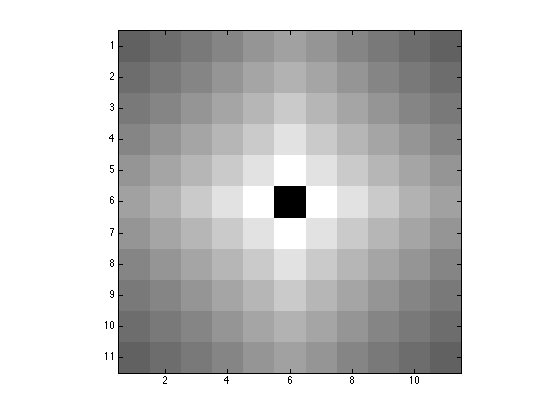
\includegraphics[width=0.7\textwidth]{valueIterationColormap.png}}
        \caption{\label{colormapValueIteration} Colormap of the $V$-values  resulting from Value 
        		Iteration for $\theta=0$ and $\gamma = 0.9$. \newline
        		The brighter the color the higher the corresponding $V$-value.}
\end{figure}

\newpage
\begin{landscape}

\begin{table}[tbp]
\centering
\begin{tabular} {c c c c c c c c c c c c}
 & 0 & 1 & 2 & 3 & 4 & 5 & 6 & 7 & 8 & 9 & 10 \\
0 & 0.000000 & 0.000002 & 0.000011 & 0.000074 & 0.000438 & 0.001730 & 0.000438 & 0.000074 & 0.000011 & 0.000002 & 0.000000\\
1 & 0.000002 & 0.000011 & 0.000075 & 0.000498 & 0.003195 & 0.013773 & 0.003195 & 0.000498 & 0.000075 & 0.000011 & 0.000002\\
2& 0.000011 & 0.000075 & 0.000498 & 0.003443 & 0.021739 & 0.117564 & 0.021739 & 0.003443 & 0.000498 & 0.000075 & 0.000011\\
3 & 0.000074 & 0.000498 & 0.003443 & 0.021739 & 0.166976 & 0.816327 & 0.166976 & 0.021739 & 0.003443 & 0.000498 & 0.000074\\
4 & 0.000438 & 0.003195 & 0.021739 & 0.166976 & 0.816327 & 10.000000 & 0.816327 & 0.166976 & 0.021739 & 0.003195 & 0.000438\\
5 & 0.001730 & 0.013773 & 0.117564 & 0.816327 & 10.000000 & 0.000000 & 10.000000 & 0.816327 & 0.117564 & 0.013773 & 0.001730\\
6 & 0.000438 & 0.003195 & 0.021739 & 0.166976 & 0.816327 & 10.000000 & 0.816327 & 0.166976 & 0.021739 & 0.003195 & 0.000438\\
7 & 0.000074 & 0.000498 & 0.003443 & 0.021739 & 0.166976 & 0.816327 & 0.166976 & 0.021739 & 0.003443 & 0.000498 & 0.000074\\
8 & 0.000011 & 0.000075 & 0.000498 & 0.003443 & 0.021739 & 0.117564 & 0.021739 & 0.003443 & 0.000498 & 0.000075 & 0.000011\\
9 & 0.000002 & 0.000011 & 0.000075 & 0.000498 & 0.003195 & 0.013773 & 0.003195 & 0.000498 & 0.000075 & 0.000011 & 0.000002\\
10 & 0.000000 & 0.000002 & 0.000011 & 0.000074 & 0.000438 & 0.001730 & 0.000438 & 0.000074 & 0.000011 & 0.000002 & 0.000000\\
\end{tabular}\\
\caption{The $V$-values for Value Iteration, with $\gamma$ = 0.1 and the prey at position (5,5). The convergence speed is 20 iterations.}
\label{valueiterationone}
\end{table}

\begin{table}[tbp]
\centering
\begin{tabular} {c c c c c c c c c c c c}
 & 0 & 1 & 2 & 3 & 4 & 5 & 6 & 7 & 8 & 9 & 10 \\
 0 & 0.0267 &  0.0502 &  0.0943 &  0.1768 &  0.3328 &  0.5332 &  0.3328 &  0.1768 &  0.0943 &  0.0502 &  0.0267\\
1 & 0.0502 &  0.0924 &  0.1769 &  0.3390 &  0.6448 &  1.0814 &  0.6448 &  0.3390 &  0.1769 &  0.0924 &  0.0502\\
2 & 0.0943 &  0.1769 &  0.3390 &  0.6498 &  1.2435 &  2.2027 &  1.2435 &  0.6498 &  0.3390 &  0.1769 &  0.0943\\
3 & 0.1768 &  0.3390 &  0.6498 &  1.2435 &  2.3977 &  4.4444 &  2.3977 &  1.2435 &  0.6498 &  0.3390 &  0.1768\\
4 & 0.3328 &  0.6448 &  1.2435 &  2.3977 &  4.4444 & 10.0000 &  4.4444 &  2.3977 &  1.2435 &  0.6448 &  0.3328\\
5 & 0.5332 &  1.0814 &  2.2027 &  4.4444 & 10.0000 &  0.0000 & 10.0000 &  4.4444 &  2.2027 &  1.0814 &  0.5332\\
6 & 0.3328 &  0.6448 &  1.2435 &  2.3977 &  4.4444 & 10.0000 &  4.4444 &  2.3977 &  1.2435 &  0.6448 &  0.3328\\
7 & 0.1768 &  0.3390 &  0.6498 &  1.2435 &  2.3977 &  4.4444 &  2.3977 &  1.2435 &  0.6498 &  0.3390 &  0.1768\\
8 & 0.0943 &  0.1769 &  0.3390 &  0.6498 &  1.2435 &  2.2027 &  1.2435 &  0.6498 &  0.3390 &  0.1769 &  0.0943\\
9 & 0.0502 &  0.0924 &  0.1769 &  0.3390 &  0.6448 &  1.0814 &  0.6448 &  0.3390 &  0.1769 &  0.0924 &  0.0502\\
10 & 0.0267 &  0.0502 &  0.0943 &  0.1768 &  0.3328 &  0.5332 &  0.3328 &  0.1768 &  0.0943 &  0.0502 &  0.0267\\
\end{tabular}\\
\caption{The $V$-values for Value Iteration, with $\gamma$ = 0.5 and the prey at position (5,5). The convergence speed is 28 iterations.}
\label{valueiteration2}
\end{table}

\begin{table}[tbp]
\centering
\begin{tabular} {c c c c c c c c c c c c}
 & 0 & 1 & 2 & 3 & 4 & 5 & 6 & 7 & 8 & 9 & 10 \\
0 &  0.4348 &  0.6065 &  0.8453 &  1.1765 &  1.6463 &  2.1169 &  1.6463 &  1.1765 &  0.8453 &  0.6065 &  0.4348\\
1 &  0.6065 &  0.8328 &  1.1750 &  1.6587 &  2.3345 &  3.0759 &  2.3345 &  1.6587 &  1.1750 &  0.8328 &  0.6065\\
2 &  0.8453 &  1.1750 &  1.6587 &  2.3415 &  3.3044 &  4.4805 &  3.3044 &  2.3415 &  1.6587 &  1.1750 &  0.8453\\
3 &  1.1765 &  1.6587 &  2.3415 &  3.3044 &  4.6737 &  6.5116 &  4.6737 &  3.3044 &  2.3415 &  1.6587 &  1.1765\\
4 &  1.6463 &  2.3345 &  3.3044 &  4.6737 &  6.5116 & 10.0000 &  6.5116 &  4.6737 &  3.3044 &  2.3345 &  1.6463\\
5 &  2.1169 &  3.0759 &  4.4805 &  6.5116 & 10.0000 &  0.0000 & 10.0000 &  6.5116 &  4.4805 &  3.0759 &  2.1169\\
6 &  1.6463 &  2.3345 &  3.3044 &  4.6737 &  6.5116 & 10.0000 &  6.5116 &  4.6737 &  3.3044 &  2.3345 &  1.6463\\
7 &  1.1765 &  1.6587 &  2.3415 &  3.3044 &  4.6737 &  6.5116 &  4.6737 &  3.3044 &  2.3415 &  1.6587 &  1.1765\\
8 &  0.8453 &  1.1750 &  1.6587 &  2.3415 &  3.3044 &  4.4805 &  3.3044 &  2.3415 &  1.6587 &  1.1750 &  0.8453\\
9 &  0.6065 &  0.8328 &  1.1750 &  1.6587 &  2.3345 &  3.0759 &  2.3345 &  1.6587 &  1.1750 &  0.8328 &  0.6065\\
10 &  0.4348 &  0.6065 &  0.8453 &  1.1765 &  1.6463 &  2.1169 &  1.6463 &  1.1765 &  0.8453 &  0.6065 &  0.4348\\
\end{tabular}\\
\caption{The $V$-values for Value Iteration, with $\gamma$ = 0.7 and the prey at position (5,5). The convergence speed is 31 iterations.}
\label{valueiteration3}
\end{table}

\begin{table}[tbp]
\centering
\begin{tabular} {c c c c c c c c c c c c}
 & 0 & 1 & 2 & 3 & 4 & 5 & 6 & 7 & 8 & 9 & 10 \\
0 &  3.8831 &  4.2915 &  4.7417 &  5.2374 &  5.7919 &  6.2513 &  5.7919 &  5.2374 &  4.7417 &  4.2915 &  3.8831\\
1 &  4.2915 &  4.7118 &  5.2281 &  5.8024 &  6.4356 &  6.9973 &  6.4356 &  5.8024 &  5.2281 &  4.7118 &  4.2915\\
2 &  4.7417 &  5.2281 &  5.8024 &  6.4401 &  7.1476 &  7.8390 &  7.1476 &  6.4401 &  5.8024 &  5.2281 &  4.7417\\
3 &  5.2374 &  5.8024 &  6.4401 &  7.1476 &  7.9362 &  8.7805 &  7.9362 &  7.1476 &  6.4401 &  5.8024 &  5.2374\\
4 &  5.7919 &  6.4356 &  7.1476 &  7.9362 &  8.7805 & 10.0000 &  8.7805 &  7.9362 &  7.1476 &  6.4356 &  5.7919\\
5 &  6.2513 &  6.9973 &  7.8390 &  8.7805 & 10.0000 &  0.0000 & 10.0000 &  8.7805 &  7.8390 &  6.9973 &  6.2513\\
6 &  5.7919 &  6.4356 &  7.1476 &  7.9362 &  8.7805 & 10.0000 &  8.7805 &  7.9362 &  7.1476 &  6.4356 &  5.7919\\
7 &  5.2374 &  5.8024 &  6.4401 &  7.1476 &  7.9362 &  8.7805 &  7.9362 &  7.1476 &  6.4401 &  5.8024 &  5.2374\\
8 &  4.7417 &  5.2281 &  5.8024 &  6.4401 &  7.1476 &  7.8390 &  7.1476 &  6.4401 &  5.8024 &  5.2281 &  4.7417\\
9 &  4.2915 &  4.7118 &  5.2281 &  5.8024 &  6.4356 &  6.9973 &  6.4356 &  5.8024 &  5.2281 &  4.7118 &  4.2915\\
10 &  3.8831 &  4.2915 &  4.7417 &  5.2374 &  5.7919 &  6.2513 &  5.7919 &  5.2374 &  4.7417 &  4.2915 &  3.8831\\\end{tabular}\\
\caption{The $V$-values for Value Iteration, with $\gamma$ = 0.9 and the prey at position (5,5). The convergence speed is 34 iterations.}
\label{valueiteration4}
\end{table}


\end{landscape}


\section{(SC) State space reduction}
In the experiments described in all following sections, unless stated otherwise, we used a state space that ...\\
\emph{ (uitleg default state space)}\\
We will refer to this state space as the ``default'' state space.\\

We elaborated on a more efficient representation for the states, and finally contrived one consisting of $30$ states, an approximately $488$ times smaller one than the default state space.  We will refer to this state space as the ``efficient''' state space. This state space... \\
\emph{(uitleg efficiente state space)}

\section{Conclusion}
Bla bla

\newpage
\appendix
\appendixpage
\section{Simulating the Environment} \label{app:firstMust}
Our program's output for the first 100 runs for the random policy predator.\\
\begin{scriptsize}
\begin{verbatim}
	Timesteps:421
	Timesteps:831
	Timesteps:476
	Timesteps:74
	Timesteps:537
	Timesteps:40
	Timesteps:468
	Timesteps:465
	Timesteps:105
	Timesteps:123
	Timesteps:227
	Timesteps:658
	Timesteps:696
	Timesteps:153
	Timesteps:426
	Timesteps:431
	Timesteps:24
	Timesteps:197
	Timesteps:517
	Timesteps:313
	Timesteps:492
	Timesteps:213
	Timesteps:457
	Timesteps:392
	Timesteps:47
	Timesteps:178
	Timesteps:459
	Timesteps:624
	Timesteps:881
	Timesteps:100
	Timesteps:244
	Timesteps:127
	Timesteps:213
	Timesteps:145
	Timesteps:45
	Timesteps:301
	Timesteps:628
	Timesteps:248
	Timesteps:88
	Timesteps:123
	Timesteps:82
	Timesteps:206
	Timesteps:181
	Timesteps:771
	Timesteps:114
	Timesteps:238
	Timesteps:118
	Timesteps:67
	Timesteps:41
	Timesteps:662
	Timesteps:27
	Timesteps:73
	Timesteps:217
	Timesteps:269
	Timesteps:382
	Timesteps:60
	Timesteps:205
	Timesteps:64
	Timesteps:133
	Timesteps:232
	Timesteps:148
	Timesteps:504
	Timesteps:113
	Timesteps:316
	Timesteps:151
	Timesteps:178
	Timesteps:53
	Timesteps:526
	Timesteps:150
	Timesteps:690
	Timesteps:490
	Timesteps:116
	Timesteps:288
	Timesteps:79
	Timesteps:163
	Timesteps:266
	Timesteps:566
	Timesteps:1194
	Timesteps:133
	Timesteps:690
	Timesteps:136
	Timesteps:121
	Timesteps:123
	Timesteps:492
	Timesteps:288
	Timesteps:185
	Timesteps:19
	Timesteps:78
	Timesteps:250
	Timesteps:42
	Timesteps:268
	Timesteps:190
	Timesteps:231
	Timesteps:393
	Timesteps:338
	Timesteps:100
	Timesteps:49
	Timesteps:653
	Timesteps:1173
	Timesteps:421
	Average timesteps over 100 trials: 296.93
	Standard deviation over 100 trials: 244.54689754728025
\end{verbatim}
\end{scriptsize}

\section{Policy Evaluation} \label{app:firstShould}
Our program's output for Policy Evaluation using a discount factor ($\gamma$) of 0.8.\\
The term ``maxValueDiff'' denotes the threshold $\theta$ should be under for the algorithm to terminate.
\begin{scriptsize}
\begin{verbatim}
Policy Evaluation, iteration number: 1; maxValueDiff = 2.173444408972901 
Policy Evaluation, iteration number: 2; maxValueDiff = 0.594273911906516 
Policy Evaluation, iteration number: 3; maxValueDiff = 0.288747386234562 
Policy Evaluation, iteration number: 4; maxValueDiff = 0.142434892859105 
Policy Evaluation, iteration number: 5; maxValueDiff = 0.077807292807347 
Policy Evaluation, iteration number: 6; maxValueDiff = 0.043989076413322 
Policy Evaluation, iteration number: 7; maxValueDiff = 0.025523868234365 
Policy Evaluation, iteration number: 8; maxValueDiff = 0.015571413160874 
Policy Evaluation, iteration number: 9; maxValueDiff = 0.009673932990005 
Policy Evaluation, iteration number: 10; maxValueDiff = 0.006050573197382 
Policy Evaluation, iteration number: 11; maxValueDiff = 0.003853977807979 
Policy Evaluation, iteration number: 12; maxValueDiff = 0.002486803847959 
Policy Evaluation, iteration number: 13; maxValueDiff = 0.001609366549420 
Policy Evaluation, iteration number: 14; maxValueDiff = 0.001044912566793 
Policy Evaluation, iteration number: 15; maxValueDiff = 0.000680717843366 
Policy Evaluation, iteration number: 16; maxValueDiff = 0.000452195511078 
Policy Evaluation, iteration number: 17; maxValueDiff = 0.000300871717137 
Policy Evaluation, iteration number: 18; maxValueDiff = 0.000201864159448 
Policy Evaluation, iteration number: 19; maxValueDiff = 0.000136221951843 
Policy Evaluation, iteration number: 20; maxValueDiff = 0.000091909267497 
Policy Evaluation, iteration number: 21; maxValueDiff = 0.000062025880297 
Policy Evaluation, iteration number: 22; maxValueDiff = 0.000042272381132 
Policy Evaluation, iteration number: 23; maxValueDiff = 0.000028863910013 
Policy Evaluation, iteration number: 24; maxValueDiff = 0.000019849447467 
Policy Evaluation, iteration number: 25; maxValueDiff = 0.000013630925504 
Policy Evaluation, iteration number: 26; maxValueDiff = 0.000009359323432 
Policy Evaluation, iteration number: 27; maxValueDiff = 0.000006460531614 
Policy Evaluation, iteration number: 28; maxValueDiff = 0.000004480328471 
Policy Evaluation, iteration number: 29; maxValueDiff = 0.000003102386442 
Policy Evaluation, iteration number: 30; maxValueDiff = 0.000002145040952 
Policy Evaluation, iteration number: 31; maxValueDiff = 0.000001489301996 
Policy Evaluation, iteration number: 32; maxValueDiff = 0.000001035209317 
Policy Evaluation, iteration number: 33; maxValueDiff = 0.000000718422800 
Policy Evaluation, iteration number: 34; maxValueDiff = 0.000000497903405 
Policy Evaluation, iteration number: 35; maxValueDiff = 0.000000344679351 
Policy Evaluation, iteration number: 36; maxValueDiff = 0.000000238380220 
Policy Evaluation, iteration number: 37; maxValueDiff = 0.000000164815624 
Policy Evaluation, iteration number: 38; maxValueDiff = 0.000000114177600 
Policy Evaluation, iteration number: 39; maxValueDiff = 0.000000079027742 
Policy Evaluation, iteration number: 40; maxValueDiff = 0.000000054656798 
Policy Evaluation, iteration number: 41; maxValueDiff = 0.000000037776286 
Policy Evaluation, iteration number: 42; maxValueDiff = 0.000000026094228 
Policy Evaluation, iteration number: 43; maxValueDiff = 0.000000018015862 
Policy Evaluation, iteration number: 44; maxValueDiff = 0.000000012433182 
Policy Evaluation, iteration number: 45; maxValueDiff = 0.000000008577363 
Policy Evaluation, iteration number: 46; maxValueDiff = 0.000000005915533 
Policy Evaluation, iteration number: 47; maxValueDiff = 0.000000004078720 
Policy Evaluation, iteration number: 48; maxValueDiff = 0.000000002811658 
Policy Evaluation, iteration number: 49; maxValueDiff = 0.000000001937877 
Policy Evaluation, iteration number: 50; maxValueDiff = 0.000000001335454 
Policy Evaluation, iteration number: 51; maxValueDiff = 0.000000000920202 
Policy Evaluation, iteration number: 52; maxValueDiff = 0.000000000634014 
Policy Evaluation, iteration number: 53; maxValueDiff = 0.000000000436804 
Policy Evaluation, iteration number: 54; maxValueDiff = 0.000000000300921 
Policy Evaluation, iteration number: 55; maxValueDiff = 0.000000000207302 
Policy Evaluation, iteration number: 56; maxValueDiff = 0.000000000142806 
Policy Evaluation, iteration number: 57; maxValueDiff = 0.000000000098375 
Policy Evaluation, iteration number: 58; maxValueDiff = 0.000000000067767 
Policy Evaluation, iteration number: 59; maxValueDiff = 0.000000000046683 
Policy Evaluation, iteration number: 60; maxValueDiff = 0.000000000032159 
Policy Evaluation, iteration number: 61; maxValueDiff = 0.000000000022154 
Policy Evaluation, iteration number: 62; maxValueDiff = 0.000000000015262 
Policy Evaluation, iteration number: 63; maxValueDiff = 0.000000000010515 
Policy Evaluation, iteration number: 64; maxValueDiff = 0.000000000007244 
Policy Evaluation, iteration number: 65; maxValueDiff = 0.000000000004991 
Policy Evaluation, iteration number: 66; maxValueDiff = 0.000000000003439 
Policy Evaluation, iteration number: 67; maxValueDiff = 0.000000000002369 
Policy Evaluation, iteration number: 68; maxValueDiff = 0.000000000001633 
Policy Evaluation, iteration number: 69; maxValueDiff = 0.000000000001125 
Policy Evaluation, iteration number: 70; maxValueDiff = 0.000000000000775 
Policy Evaluation, iteration number: 71; maxValueDiff = 0.000000000000534 
Policy Evaluation, iteration number: 72; maxValueDiff = 0.000000000000368 
Policy Evaluation, iteration number: 73; maxValueDiff = 0.000000000000254 
Policy Evaluation, iteration number: 74; maxValueDiff = 0.000000000000175 
Policy Evaluation, iteration number: 75; maxValueDiff = 0.000000000000120 
Policy Evaluation, iteration number: 76; maxValueDiff = 0.000000000000083 
Policy Evaluation, iteration number: 77; maxValueDiff = 0.000000000000057 
Policy Evaluation, iteration number: 78; maxValueDiff = 0.000000000000039 
Policy Evaluation, iteration number: 79; maxValueDiff = 0.000000000000027 
Policy Evaluation, iteration number: 80; maxValueDiff = 0.000000000000019 
Policy Evaluation, iteration number: 81; maxValueDiff = 0.000000000000013 
Policy Evaluation, iteration number: 82; maxValueDiff = 0.000000000000009 
Policy Evaluation, iteration number: 83; maxValueDiff = 0.000000000000006 
Policy Evaluation, iteration number: 84; maxValueDiff = 0.000000000000004 
Policy Evaluation, iteration number: 85; maxValueDiff = 0.000000000000003 
Policy Evaluation, iteration number: 86; maxValueDiff = 0.000000000000002 
Policy Evaluation, iteration number: 87; maxValueDiff = 0.000000000000002 
Policy Evaluation, iteration number: 88; maxValueDiff = 0.000000000000001 
Policy Evaluation, iteration number: 89; maxValueDiff = 0.000000000000001 
Policy Evaluation, iteration number: 90; maxValueDiff = 0.000000000000002 
Policy Evaluation, iteration number: 91; maxValueDiff = 0.000000000000001 
Policy Evaluation, iteration number: 92; maxValueDiff = 0.000000000000000 
Policy Evaluation, iteration number: 93; maxValueDiff = 0.000000000000000 
Policy Evaluation, iteration number: 94; maxValueDiff = 0.000000000000000 
Policy Evaluation, iteration number: 95; maxValueDiff = 0.000000000000000 
Policy Evaluation, iteration number: 96; maxValueDiff = 0.000000000000000 
Policy Evaluation, iteration number: 97; maxValueDiff = 0.000000000000000 
Policy Evaluation, iteration number: 98; maxValueDiff = 0.000000000000000 
Policy Evaluation, iteration number: 99; maxValueDiff = 0.000000000000000 
Policy Evaluation, iteration number: 100; maxValueDiff = 0.000000000000000 
Policy Evaluation, iteration number: 101; maxValueDiff = 0.000000000000000 
Policy Evaluation, iteration number: 102; maxValueDiff = 0.000000000000000 
Policy Evaluation, iteration number: 103; maxValueDiff = 0.000000000000000 
Policy Evaluation, iteration number: 104; maxValueDiff = 0.000000000000000 
Policy Evaluation, iteration number: 105; maxValueDiff = 0.000000000000000 
Policy Evaluation, iteration number: 106; maxValueDiff = 0.000000000000000 
Policy Evaluation, iteration number: 107; maxValueDiff = 0.000000000000000 
Policy Evaluation, iteration number: 108; maxValueDiff = 0.000000000000000 
Policy Evaluation, iteration number: 109; maxValueDiff = 0.000000000000000 
Policy Evaluation, iteration number: 110; maxValueDiff = 0.000000000000000 
Policy Evaluation, iteration number: 111; maxValueDiff = 0.000000000000000 
\end{verbatim}
\end{scriptsize}


\end{document}
